\documentclass{article}

\usepackage{graphicx}
\usepackage{tikz}
\usepackage{tikzsymbols}
\usetikzlibrary{calc,patterns,shapes.geometric}
\pagestyle{empty}
\usepackage[margin=0pt]{geometry}
\geometry{papersize={14in,12in}}

\def\centerarc[#1](#2)(#3:#4:#5){\draw[#1] ($(#2)+({#5*cos(#3)},{#5*sin(#3)})$) arc (#3:#4:#5);}

\begin{document}
	\begin{figure}
		\centering
		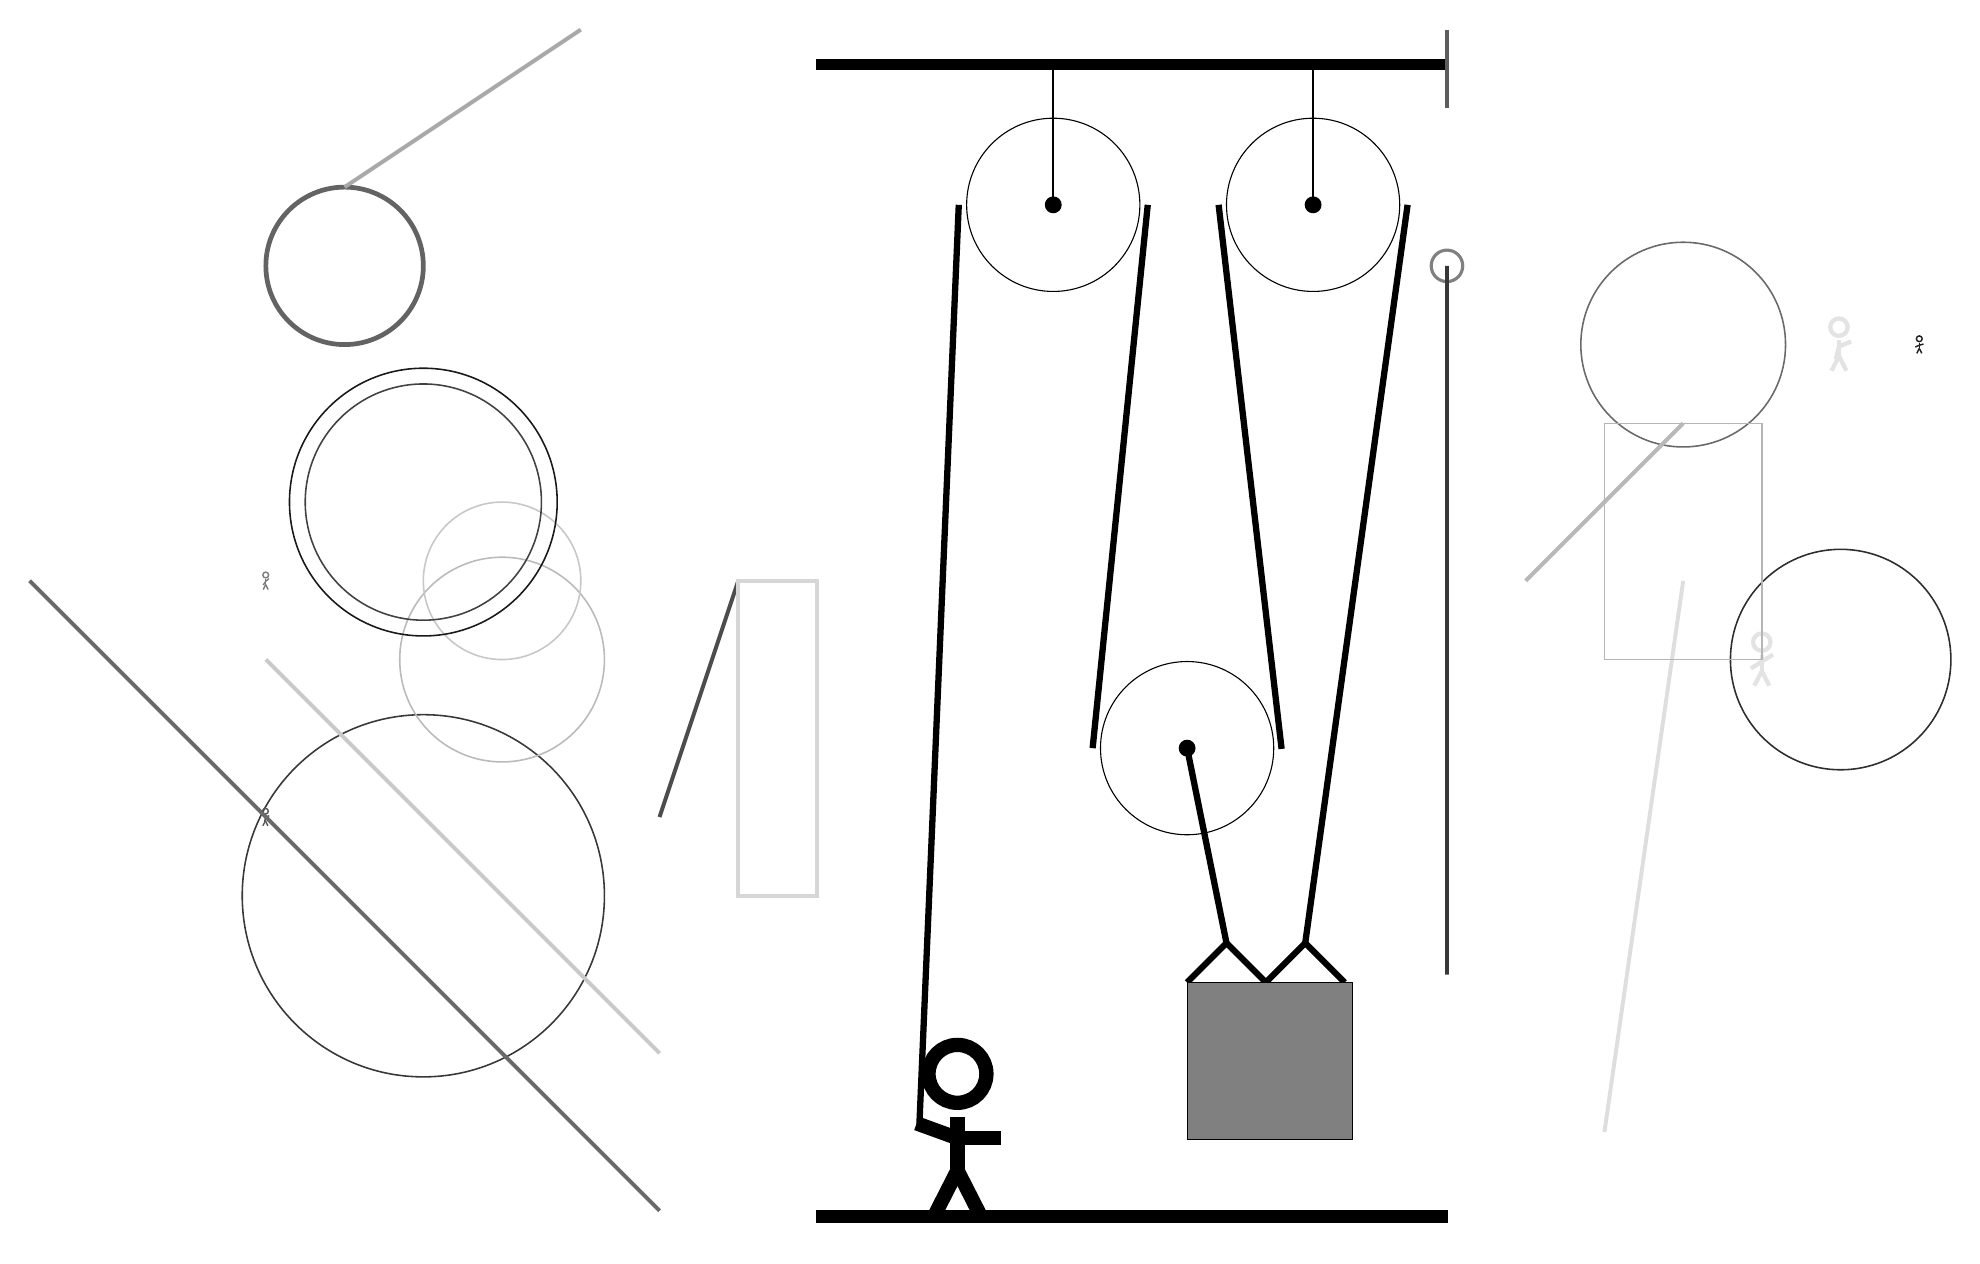
\begin{tikzpicture}
			%%%%% START %%%%%
			
			\draw[fill=black] (-2, 11.5) rectangle (6, 11.625);
			
			\draw [line width=0.2mm, color=black!78](-7, 1) circle (2.3);
			
			\draw [line width=0.6mm, color=black!61](-8, 9) circle (1.0);
			\draw [line width=0.2mm, color=black!27](-6, 4) circle (1.3);
			\draw[line width=0.5mm, color=black!64](6, 11) -- (6, 12);
			\node[line width=0.2mm, color=black!66] at (-9, 2) {\Strichmaxerl[1][80][28]};
			\draw[line width=0.5mm, color=black!59](-4, -3) -- (-12, 5);
			
			\node[line width=0.3mm, color=black!51] at (-9, 5) {\Strichmaxerl[1][55][43]};
			\draw [line width=0.2mm, color=black!22](-6, 5) circle (1.0);
			\node[line width=0.5mm, color=black!88] at (12, 8) {\Strichmaxerl[1][25][16]};
			
			\draw [line width=0.2mm, color=black!59](9, 8) circle (1.3);
			\draw[line width=0.5mm, color=black!21](-4, -1) -- (-9, 4);
			\node[line width=0.2mm, color=black!11] at (10, 4) {\Strichmaxerl[3][33][31]};
			\draw [line width=0.4mm, color=black!50](6, 9) circle (0.2);
			\draw [line width=0.2mm, color=black!82](11, 4) circle (1.4);
			\draw [line width=0.2mm, color=black!74](-7, 6) circle (1.5);
			\draw[line width=0.5mm, color=black!70](-3, 5) -- (-4, 2);
			\draw[line width=0.5mm, color=black!16] (-2, 5) rectangle (-3, 1);
			
			\draw [line width=0.6mm, color=black!78](10, 9) circle (0.0);
			\draw[line width=0.5mm, color=black!28](7, 5) -- (9, 7);
			
			\draw[line width=0.4mm, color=black!78] (6, 0) rectangle (6, 9);
			\draw [line width=0.2mm, color=black!90](-7, 6) circle (1.7);
			
			\draw[line width=0.5mm, color=black!13](8, -2) -- (9, 5);
			
			\node[line width=0.5mm, color=black!11] at (11, 8) {\Strichmaxerl[3][76][22]};
			\draw [line width=0.4mm, color=black!78](-7, 9) circle (0.0);
			\draw[line width=0.5mm, color=black!34](-5, 12) -- (-8, 10);
			\draw[line width=0.2mm, color=black!29] (8, 7) rectangle (10, 4);
			
			\draw (1, 9.775) circle (1.1);
			\draw[fill=black] (1, 9.775) circle (0.1);
			\draw[thick] (1, 9.775) -- (1, 11.5);
			
			\draw (4.3, 9.775) circle (1.1);
			\draw[fill=black] (4.3, 9.775) circle (0.1);
			\draw[thick] (4.3, 9.775) -- (4.3, 11.5);
			
			\draw (2.7, 2.875) circle (1.1);
			\draw[fill=black] (2.7, 2.875) circle (0.1);
			
			\draw[line width=0.8mm]  (2.7, -0.1) -- (3.2, 0.4) -- (3.7, -0.1) -- (4.2, 0.4) -- (4.7, -0.1);
			\draw[fill=black!50] (2.7, -0.1) rectangle (4.8, -2.1);
			
			\draw[line width=0.8mm](-0.7, -1.9) -- (-0.2, 9.775);
			\centerarc[line width=0.8mm](1, 9.775)(0:180:1.2000000000000002);
			\draw[line width=0.8mm](2.2, 9.775) -- (1.5, 2.875);
			\centerarc[line width=0.8mm](2.7, 2.875)(180:370:1.2000000000000002);
			\draw[line width=0.8mm] (3.9, 2.865) -- (3.1, 9.775);
			\centerarc[line width=0.8mm](4.3, 9.775)(0:180:1.2000000000000002);
			\draw[line width=0.8mm](4.2, 0.4) -- (5.5, 9.775);
			\draw[line width=0.8mm] (3.2, 0.4) -- (2.7, 2.875);
			
			\node at (-0.2, -2) {\Strichmaxerl[10][-20][0]};
			
			\draw[fill=black] (-2, -3) rectangle (6, -3.15);
			
			%%%%% END %%%%%
		\end{tikzpicture}
	\end{figure}	
\end{document}